\apendice{Plan de Proyecto Software}

\section{Introducción}
En este apéndice del anexo se plasmará toda la información de seguimiento (sprints de Scrum),el análisis de costes y viabilidad del proyecto.


\section{Planificación temporal}
Al comenzar el proyecto se determinó que se utilizaría una metodología ágil para hacer el desarrollo del proyecto pero esta decisión ha terminado siendo un handicap producido por la falta de documentación y la dudosa credibilidad de la mayoría de páginas webs y documentación, se traducido en un gran coste temporal.
Por otro lado, el redactar el proyecto en \LaTeX{} desde la plataforma de Overleaf no refleja el tiempo real invertido puesto que no se realizan cambios en el repositorio de forma automática, hasta que compilo, descargo y actualizo el repositorio manualmente.

Ante todo, se ha intentado seguir un mínimo de pautas \textbf{Scrum} pese a no existir un grupo de trabajo real con unas tareas diarias y roles definidos:
\begin{itemize}
    \item Las tareas fueron siempre semanales en forma de <<sprints>>.
    \item Al finalizar el sprint se hace la entrega del trabajo elaborado en la semana y se determinan las próximas tareas.
    \item Tras determinar las tareas se definen los <<milestones>> y los <<issues>>.
    \item Para hacer el seguimiento de las tareas se ha utilizado en tablero \textbf{Kanban} de \textbf{ZenHub}.
    \item Tras finalizar el sprint se puede comprobar el trabajo mediante los  \textit{gráficos burndown}.
\end{itemize}

Las reuniones de trabajo han sido consensuadas y planificadas los jueves de cada semana, con el siguiente resultado:

\begin{figure}
    \centering
    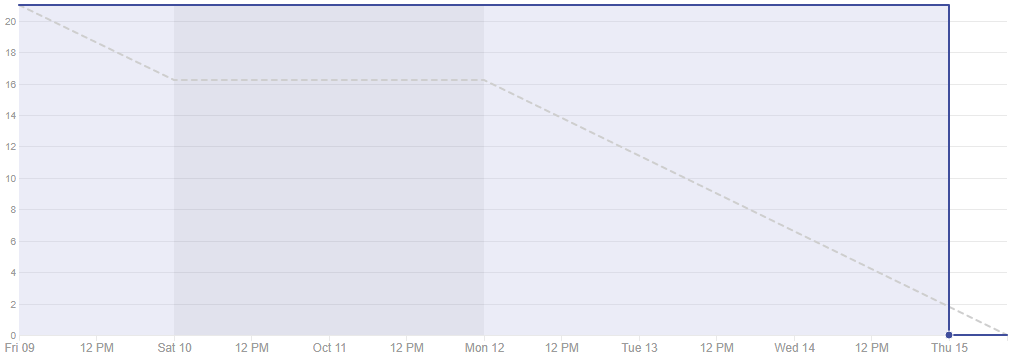
\includegraphics[width=0.7\textwidth]{img/BurnDown/1.PNG}
    \caption{Gráfico Burndown sprint1. } \label{BD1}
    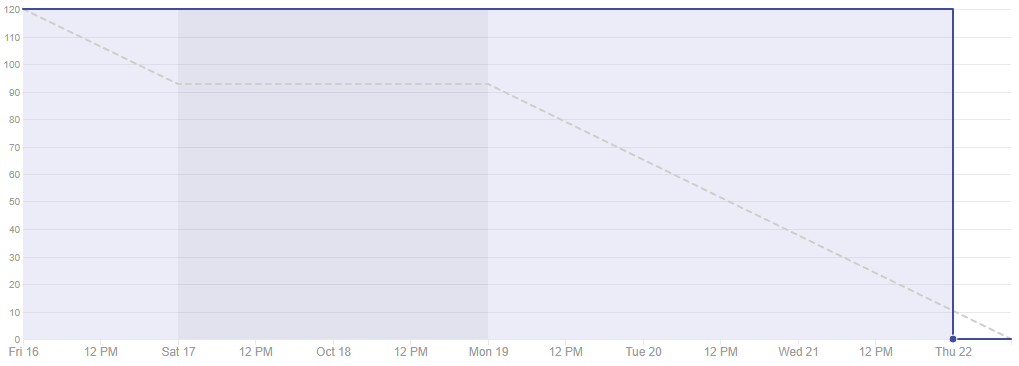
\includegraphics[width=0.7\textwidth]{img/BurnDown/2.PNG}
    \caption{Gráfico Burndown sprint2. } \label{BD2}
\end{figure}

\subsection{Sprint 00 - 01/10/2020 - 08/10/2020}
En la primera reunión nos reunimos Álvar Arnaiz González y yo. En ella hice la propuesta de temática del TFG y, además expuse diferentes ideas y enfoques sobre el proyecto en la que se determinó a grandes rasgos la posible viabilidad del proyecto.
Los objetivos de este sprint fueron la búsqueda de repositorios y otros proyectos para tomar ideas o si era posible hacer algún fork. También, el estudio la estructura del proyecto y herramientas software e interfaces a utilizar.

\subsection{Sprint 01 - 09/10/2020 - 15/10/2020}
Tras determinar el enfoque final de proyecto, se determinó que los objetivos de este sprint fueron la búsqueda de información relevante, otros proyectos y recursos que puedan servir de utilidad como pueden ser APIS. Se propusieron algunas APIS online para realizar pruebas.
Las tareas se descompusieron en unidades pequeñas de trabajo para poder afrontarlas semanalmente mediante sprints.



\subsection{Sprint 02 - 16/10/2020 - 22/10/2020}
Los objetivos de este sprint fueron el buscar repositorios, APIS, servicios y tecnologías con las que darle forma al proyecto. Se decidió generar algún tipo de aplicación desde la que poder controlar la instalación haciéndola más amigable y con mejor capacidad de interacción. Se investigan opciones.


\subsection{Sprint 03 - 23/10/2020 - 29/10/2020}
Los objetivos de este sprint fueron determinar los componentes hardware necesarios para completar el proyecto y se realiza la compra de material.
Se presenta la opción de hacer una aplicación mediante el Bot de Telegram.

\begin{figure}
    \centering
    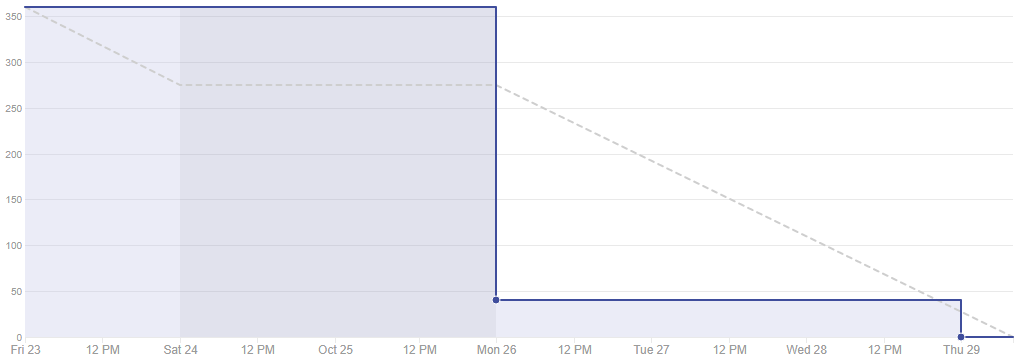
\includegraphics[width=0.7\textwidth]{img/BurnDown/3.PNG}
    \caption{Gráfico Burndown sprint3. } \label{BD3}
    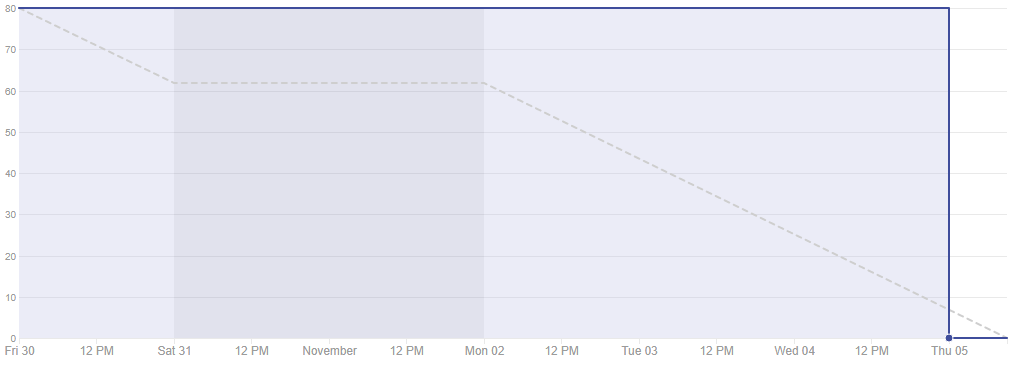
\includegraphics[width=0.7\textwidth]{img/BurnDown/4.PNG}
    \caption{Gráfico Burndown sprint4. } \label{BD4}
\end{figure}

\subsection{Sprint 04 - 30/10/2020 - 05/10/2020}
Se incorpora D.Alejandro Merino Gómez al que se le presenta el proyecto y se le concede acceso a los repositorios para que pueda co-tutorizar el proyecto.
Los objetivos de este sprint fueron la instalación física de la instalación y la tirada de cable inicial.


\subsection{Sprint 05 - 06/11/2020 - 12/11/2020}
Se repasan los cambios propuestos y se incluyen nuevos. Se hace el seguimiento de la instalación y se comentan las fotos y el estado de la instalación.
Los objetivos de este sprint son todos aquellos que sean necesarios para la adecuación del software al proyecto. Estoy incluye la actualización del sistema operativo e instalación de software adicional. Además se deben valorar opciones para controlar los GPIO.

\begin{figure}
    \centering
    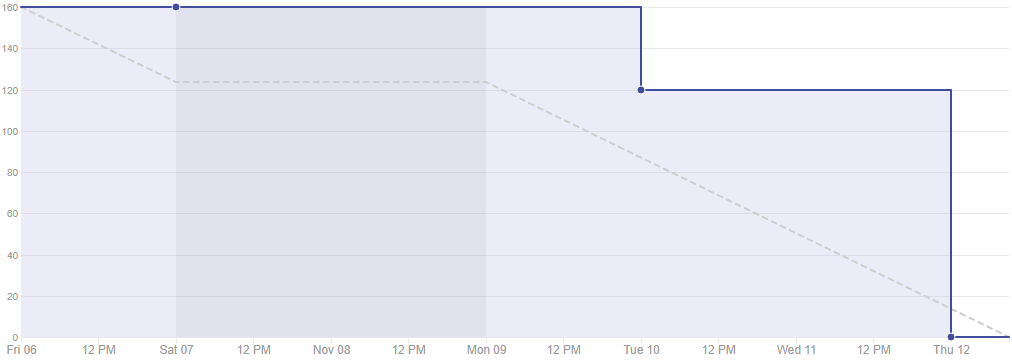
\includegraphics[width=0.7\textwidth]{img/BurnDown/5.PNG}
    \caption{Gráfico Burndown sprint5. } \label{BD5}
    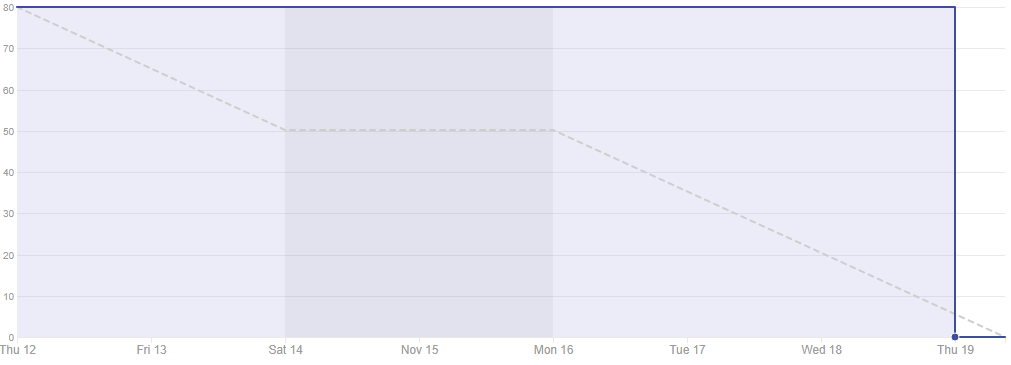
\includegraphics[width=0.7\textwidth]{img/BurnDown/6.PNG}
    \caption{Gráfico Burndown sprint6. } \label{BD6}
\end{figure}

\subsection{Sprint 06 - 13/11/2020 - 19/11/2020}
Se compone un tablero de pruebas de forma que se puede controlar el encendido de una bombilla desde nuestra Raspberry Pi. Se graba un vídeo explicativo y se diseñan unos diagramas explicativos.


\subsection{Sprint 07 - 20/11/2020 - 26/11/2020}
Se realiza una investigación sobre como se puede implantar el bot en nuestro proyecto, se realiza el primer código de pruebas y se presentan las primeras pruebas con el bot. Además, se proponen correccionesen la redacción.

\begin{figure}
    \centering
    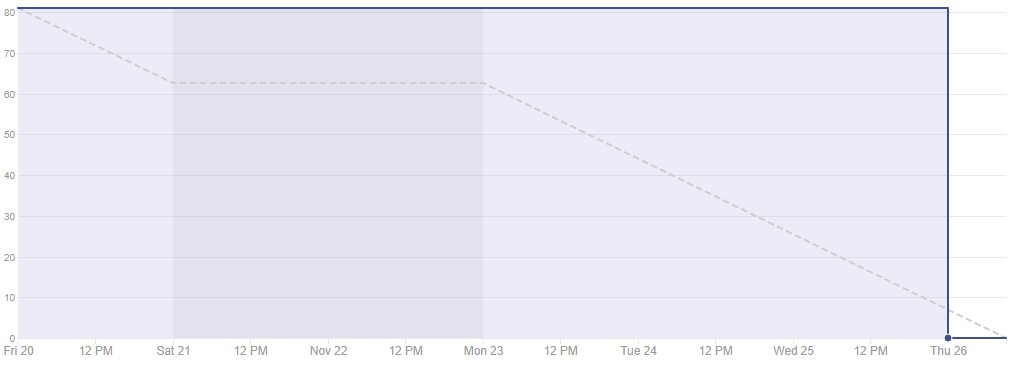
\includegraphics[width=0.7\textwidth]{img/BurnDown/7.PNG}
    \caption{Gráfico Burndown sprint7. } \label{BD7}
    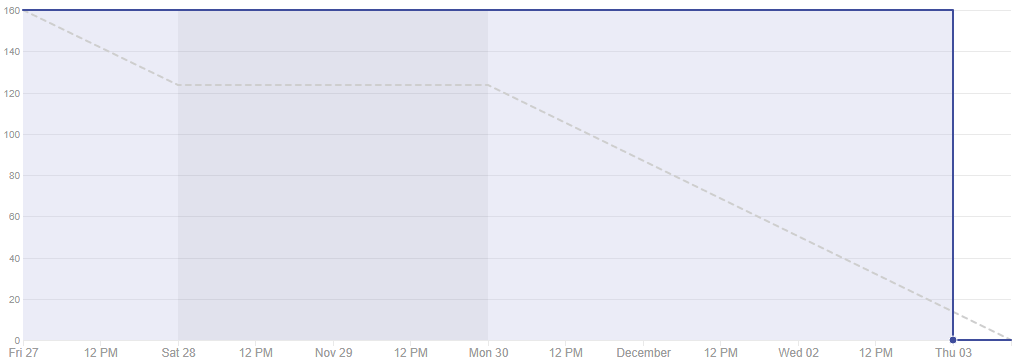
\includegraphics[width=0.7\textwidth]{img/BurnDown/8.PNG}
    \caption{Gráfico Burndown sprint8. } \label{BD8}
\end{figure}

\subsection{Sprint 08 - 27/11/2020 - 03/12/2020}
Se genera la primera automatización de la parte automática del proyecto utilizando CRON.
Se implanta los scripts finales de geolocalización y cálculo de temperaturas que utilizaremos para generar el control de nuestro sistema domótico.
Se presentan las primeras funcionalidades del bot, se proponen cambios y mejoras.


\subsection{Sprint 09 - 04/12/2020 - 10/12/2020}
Se proponen revisan las funcionalidades y se proponen cambios y mejoras en estas. 

\begin{figure}
    \centering
    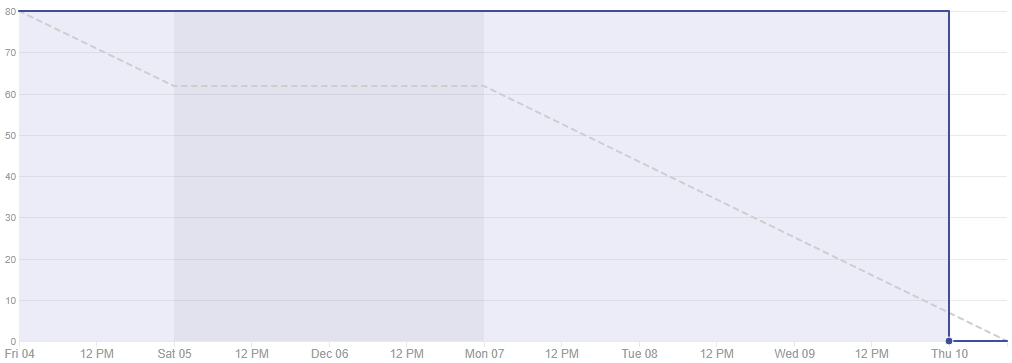
\includegraphics[width=0.7\textwidth]{img/BurnDown/9.PNG}
    \caption{Gráfico Burndown sprint9. } \label{BD9}
    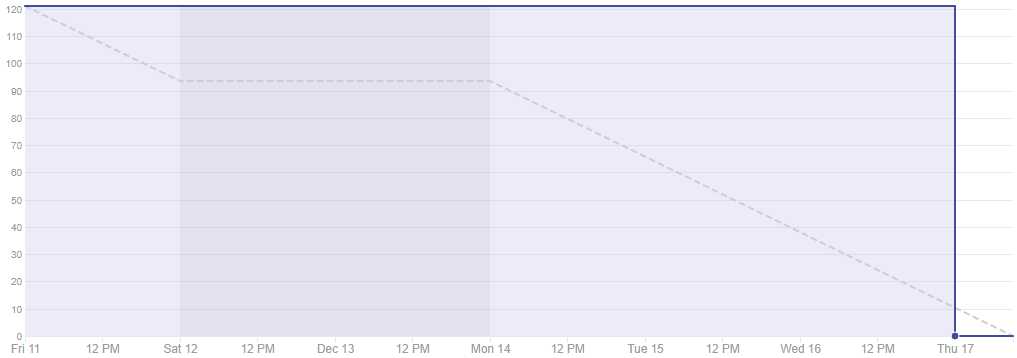
\includegraphics[width=0.7\textwidth]{img/BurnDown/10.PNG}
    \caption{Gráfico Burndown sprint10. } \label{BD10}
\end{figure}

\subsection{Sprint 10 - 11/12/2020 - 17/12/2020}
Se comprueban las funcionalidades proponiendo cambios funcionales y de estilos de forma que se pueda interactuar contra el bot y se muestren los mensajes en un formato más atractivo.También se propone unificar las rutas de trabajo de los diferentes scripts.



\subsection{Sprint 11 - 18/12/2020 - 24/12/2020}
Se propone dividir el código por funcionalidades (obtención de información de la web, y por otro lado, modificación de archivos del sistema)
Se proponen cambios en la redacción a implementar en el sprint 12.
\begin{figure}
    \centering
    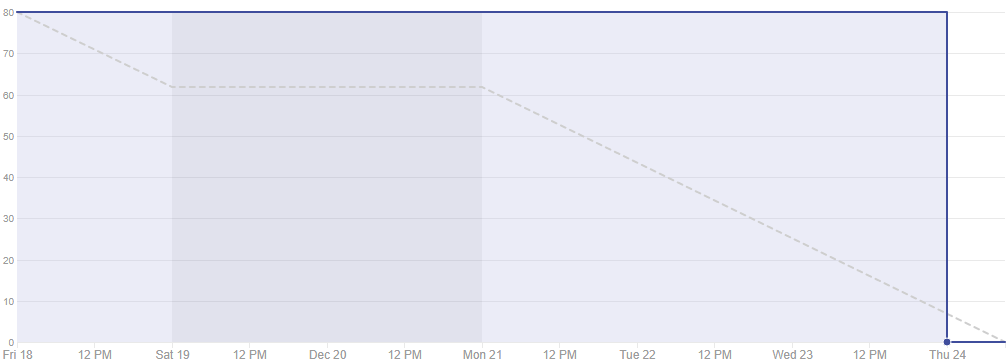
\includegraphics[width=0.7\textwidth]{img/BurnDown/11.PNG}
    \caption{Gráfico Burndown sprint11. } \label{BD11}
\end{figure}


\subsection{Sprint 12 - 30/12/2020 - 06/01/2021}
Cambios en el texto del TFG y redacción del mismo.

\subsection{Sprint 13 - 07/01/2020 - 13/01/2020}
Redacción del proyecto del TFG y grabado de vídeos.

\subsection{Sprint 14 - 14/01/2020 - 20/01/2020}
Edición de vídeos y entrega.



\section{Estudio de viabilidad}

\subsection{Viabilidad económica}

\subsection{Viabilidad legal}


